\documentclass[aspectratio=169]{beamer}
\usepackage{textcomp}
\usepackage{booktabs}
\usepackage{graphicx}
\usepackage{hyperref}
\usepackage{amsmath}
\hypersetup{
    colorlinks=true,
    linkcolor=magenta,
    filecolor=magenta,
    urlcolor=magenta,
    }
\title{Design a liquid hydrogen powered aircraft\\with surrogate models}
\author{Matthias De Lozzo}
\institute{matthias.delozzo[at]irt-saintexupery[dot]com}
\date{09-10/2022 @ ModIA @ INSA Toulouse}


\begin{document}

\frame{\titlepage}

\begin{frame}{Introduction}
    \begin{itemize}
        \item Goal: design a liquid hydrogen powered aircraft (a/c) from a numerical simulator\footnote{The study case is kindly provided by Thierry Druot, Pre-Project Research Engineer at Airbus, seconded to ENAC.
              Thanks, Thierry!}.
        \item Three problems:
        \begin{enumerate}
            \item Design an a/c in a deterministic context.
            \item Quantify the uncertainties impacting the a/c design.
            \item Design an a/c in an uncertain context.
        \end{enumerate}
        \item Constraint: the number of calls to the numerical simulator is limited.\\
              $\Rightarrow$ a surrogate model is required.
        \item Tools: the Python libraries
        \begin{itemize}
            \item MARILib, for multidisciplinary airplane research,
            \item scikit-learn, for machine learning,
            \item OpenTURNS\@, for uncertainty quantification,
            \item GEMSEO, to set the design problem and orchestrate the workflow,
            \item NumPy and SciPy for general scientific computing capabilities,
        \end{itemize}
        \item Deliverable: a report (10 to 20 pages) with introduction, sections, conclusion, images, \ldots but not code.
              Do not forget context, explanations and style checking!
    \end{itemize}
\end{frame}

\section{Case study}\label{sec:use-case}

\begin{frame}{Contents}
    \tableofcontents
\end{frame}

\begin{frame}{Contents}
    \tableofcontents[currentsection]
\end{frame}

\begin{frame}{Context}
    Hydrogen (H2) is a candidate to replace kerosene for future airplanes because it does not emit carbon dioxide when burning.
    \begin{block}{Study}
    We seek to evaluate the impact of the use of liquid hydrogen (LH2) in place of kerosene on the design and performances of a turbofan airplane.
    \end{block}
    \begin{columns}
    \begin{column}{0.6\textwidth}
    \begin{exampleblock}{Use case}
    We will focus on the design of an A320-type aircraft (a/c)
    with the same requirements as the classical kerosene A320
    but powered with liquid hydrogen.
    \end{exampleblock}
    \end{column}
    \begin{column}{0.4\textwidth}
        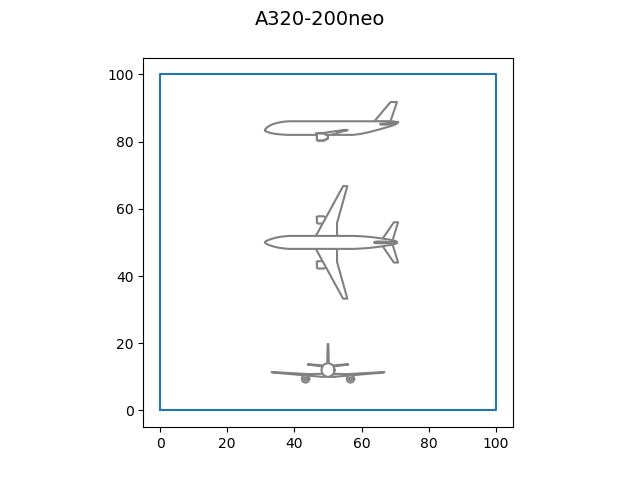
\includegraphics[width=\linewidth]{lh2pac_2}
    \end{column}
    \end{columns}
\end{frame}
\begin{frame}{The 3 main problems with liquid hydrogen}
    Because of the airborne LH2 storage:
    \begin{enumerate}
        \item The very low \textbf{temperature} of LH2 (around 20 K, -253\textdegree C) requires very specific fuel system to take it from the tank and feed the engine at ambient temperature.
        \item The \textbf{volume} of the tank is about 4 time bigger than with kerosene for an equivalent amount of internal energy.
        \item The \textbf{weight} of tank is important due the necessary high level of insulation.
    \end{enumerate}
    Point 1 is out of the scope of this study.

    Points 2 and 3 are linked to the level of maturity of storing technology.
\end{frame}
\begin{frame}{Technological level of LH2 tanking system}
    \begin{itemize}
        \item Gravimetric index: $\textrm{LH2}_{\textrm{mass}}/(\textrm{LH2}_{\textrm{mass}}+\textrm{Tank}_{\textrm{mass}})$
        \item Volumetric index: $\textrm{LH2}_{\textrm{volume}}/(\textrm{LH2}_{\textrm{volume}}+\textrm{Tank}_{\textrm{volume}})$
    \end{itemize}
    \begin{columns}
        \begin{column}{0.5\linewidth}
            \begin{table}
                \centering
                \begin{tabular}{lcc}
                    \toprule
                    & 2021 & 2030 \\
                    \midrule
                    GI & 0.1 & 0.3 \\
                    VI & 0.606 & 0.845 \\
                    \bottomrule
                \end{tabular}
                \label{tab:indices}
            \end{table}
        \end{column}
        \begin{column}{0.5\linewidth}
            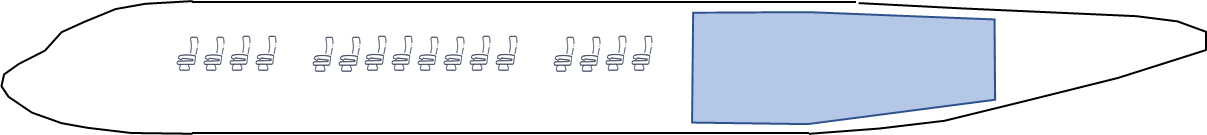
\includegraphics[width=\linewidth]{lh2pac_1}\\
            Put the tank in the rear fuselage.
        \end{column}
    \end{columns}
    $\Rightarrow$ Share the available length inside the fuselage between passengers and LH2 tank.

    $\Rightarrow$ Lengthen the fuselage of the kerosene a/c up to a certain limit.

    We will express a fuselage in terms of the ratio length/diameter
    and will take its maximum value from the A340-600 which is considered has an extreme.
\end{frame}
\begin{frame}{The performances of the A320}
    \footnotesize
    \begin{itemize}
    \item Nominal seat capacity = 150 pax (passengers)
    \item Nominal range = 3000 NM (1 Nautical Mile = 1852 m)
    \item Cruise speed = Mach 0.78
    \item Maximum Take Off Weight (MTOW) = 77000 kg
    \item Maximum Landing Weight (MLW) = 65000 kg
    \item Engine maximum thrust = 120 kN (103 Newtons)
    \item Engine Bypass Ratio (BPR) = 9 (ratio of cold flow over hot flow for a turbofan)
    \item Wing area = 122 m\textsuperscript{2}
    \item Wing aspect ratio = 9 (wing\_span\textsuperscript{2} / wing\_area)
    \item Fuselage aspect ratio = 11.0 (fuselage\_length / fuselage\_height, maximum is 13.4)
    \item Maximum Take Off Field Length (TOFL) sea level, temperature ISA+15, MTOW = 2200 m
    \item Maximum Approach speed sea level, temperature ISA, MLW = 137 kt ($\approx$ 253 km/h)
    \item Minimum Vertical speed Top Of Climb (TOC), 97\% MTOW, cruise speed, ISA, Max Climb Rating (MCL) = 300 ft/min ($\approx$ 1.5 m/s)
    \item Minimum Vertical speed Top Of Climb (TOC), 97\% MTOW, cruise speed, ISA, Max Cruise Rating (MCR) = 0 ft/min
    \item One engine inoperative minimum climb path, 97\% MTOW, ISA, Maxi Continuous Rating (MCN) = 1.1\%
    \item Maximum Time To Climb to cruise altitude, Maxi Climb Rating (MCL) = 25 min
    \end{itemize}
\end{frame}
\begin{frame}{A LH2 powered a/c for 2030}
    \begin{block}{Passenger capacity wins over range}
    Range of 3000 NM could not be achieved with 150 passengers on board.
    Number of passengers, range or both must be reduced.
    After having discussed with marketing team,
    engineers have chosen to keep the passenger capacity and reduce the range to 1800 NM\@.
    \end{block}
    \begin{block}{2030 horizon}
    Around 10 years to develop and certify $\Rightarrow$ 2030 technological level,
    assuming that there will be no significant impact on the engine characteristics and performances.
    \end{block}
    \begin{block}{Find the "best" LH2 powered A320-like a/c}
        \begin{itemize}
            \item Minimize its Maximum Take Off Weight (MTOW).
            \item Satisfy the same operational constraints as the kerosene A320 (except for the range).
        \end{itemize}
    \end{block}
\end{frame}
\begin{frame}{The design problem - Objective}
    Minimize the MTOW (Maximum Take Off Weight).
\end{frame}
\begin{frame}{The design problem - Design parameters}
    \begin{itemize}
        \item Engine maximum thrust: 100 kN $\leq$ thrust $\leq$ 150 kN
        \item Engine Bypass Ratio (BPR): 5 $\leq$ BPR $\leq$ 12
        \item Wing area: 120 m\textsuperscript{2} $\leq$ area $\leq$ 200 m\textsuperscript{2}
        \item Wing aspect ratio: 7 $\leq$ ar $\leq$ 12
    \end{itemize}
\end{frame}
\begin{frame}{The design problem - Operational Constraints}
    \begin{itemize}
        \item Take Off Field Length: TOFL $\leq$ 2200 m
        \item Approach speed: VAPP $\leq$ 137 kt
        \item Vertical speed MCL rating: 300 ft/min $\leq$ VZ\_MCL
        \item Vertical MCR rating: 0ft/min $\leq$ VZ\_MCR
        \item One engine inoperative climb path: 1.1\% $\leq$ OEI\_PATH
        \item Time To Climb to cruise altitude: TTC $\leq$ 25 min
        \item Fuselage Aspect Ratio: FAR $\leq$ 13.4
    \end{itemize}
\end{frame}
\begin{frame}{The design problem - Uncertain technological parameters}
    \begin{enumerate}
        \item Tank gravimetric index $\sim\mathcal{T}(0.25, 0.3, 0.305)$
        \item Tank volumetric index $\sim\mathcal{T}(0.8, 0.845, 085)$
        \item Aerodynamic efficiency factor $\sim\mathcal{T}(0.99, 1., 1.03)$
        \item Propulsion efficiency factor $\sim\mathcal{T}(0.99, 1., 1.03)$
        \item Structure efficiency factor $\sim\mathcal{T}(0.99, 1., 1.03)$
    \end{enumerate}
    where $\mathcal{T}(l,m,u)$ is the triangular distribution with mode $m$ and bounds $l$ and $u$.

    Note that these probability distributions are not symmetrical as it is always easier to make something less efficient than expected.

    The efficiency factors 3, 4 and 5 represent the part of indetermination that relies in any creative activity.
    They are related to the main technical areas involved in a/c design.
\end{frame}

\section{Problems}\label{sec:problems}

\begin{frame}{Contents}
    \tableofcontents[currentsection]
\end{frame}

\begin{frame}[fragile]{Numerical simulator}
    To solve the problem,
    a Python function is provided to compute the criterion and the operational constraints
    from the design and technological parameters:

    \texttt{data = fct\_turbofan\_h2(techno, design, mode)}

    This function packages a dedicated Python script which is an application of \href{https://github.com/marilib/MARILib_obj}{MARILib} (Multidisciplinary Airplane Research Integrated Library) developed at \href{https://www.enac.fr/en}{ENAC} to support Airplane Conceptual Design Teaching and some research activities\footnote{
    Thierry Druot, Mathieu Belleville, Pascal Roches, Fran\c{c}ois Gallard, Nicolas Peteilh, et al. A Multidisciplinary Airplane Research Integrated Library With Applications To Partial Turboelectric Propulsion. AIAA Aviation 2019 Forum, Jun 2019, Dallas, United States. \href{https://hal-enac.archives-ouvertes.fr/hal-02160977}{hal-02160977}
    }.

    \begin{alertblock}{Computational cost}
        The execution time of this function is low for academic reasons
        but must be considered as high for representativeness ones.
        The number of calls to the function is limited.
    \end{alertblock}
\end{frame}
\begin{frame}{Global problem}
    The global problem aims to
    minimize the MTOW
    while ensuring operational constraints
    by varying four design parameters.

    By the way, the a/c design takes place in an uncertain environment where the technological choices can be probabilized.

    In the following, we will note $$f:x,u\mapsto f(x,u)$$ the MARILib-based model of a liquid hydrogen powered model where $x$ are the design parameters and $u$ the uncertain ones.
\end{frame}
\begin{frame}{Problem 1: design an a/c in a deterministic context}
    \begin{enumerate}
        \item As the number of calls to $f$ is limited,
              we will create a surrogate model $\hat{g}$ of $$g:x\mapsto f(x,u_{\textrm{fixed}})$$
              where $u_{\textrm{fixed}}$ could be the mean value for instance,
              or the pessimistic values of the uncertain technological parameters\footnote{We could solve the problem with each option and compare the optimal designs.}.
        \item Then,
              we will use this surrogate model in an optimization process to minimize the objective whilst ensuring the constraints by varying the design parameters.
    \end{enumerate}
As $f$ is actually not expensive for academic reasons,
we will solve the problem  compare the optima found with $\hat{g}$ and $g$.
\end{frame}
\begin{frame}{Problem 2: quantifying the uncertainties in the a/c design}
    \begin{enumerate}
        \item As the number of calls to $f$ is limited,
              we will create a surrogate model $\hat{h}$ of $$h:x\mapsto h(x_{\textrm{fixed}},u)$$
              where $x_{\textrm{fixed}}$ could be the optimum found in Problem 1,
              or the center of the design space\footnote{We could solve the problem with each option and compare the results.}.
        \item Then,
              we will use this surrogate model to quantify the output uncertainties (mean, variance, boxplots, sensitivity indices, \ldots).
    \end{enumerate}
\end{frame}
\begin{frame}{[Optional] Problem 3: design an a/c in an uncertain context}
    \begin{enumerate}
        \item As the number of calls to $f$ is limited,
              we will create a surrogate model $\hat{f}$ of $$f:x,u\mapsto f(x,u)$$
        \item Then,
              we will use this surrogate model in an robust optimization process to minimize the mean objective whilst ensuring the constraints with high probability by varying the design parameters.
    \end{enumerate}
\end{frame}

\section{Quickstart}

\begin{frame}{Contents}
    \tableofcontents[currentsection]
\end{frame}

\begin{frame}{Prerequisites}
    \begin{itemize}
        \item Clone the branch \textit{modia} of the project \href{https://gitlab.com/MatthiasDeLozzo/n2pac/-/tree/modia}{LH2PAC}:
            \begin{itemize}
                \item SSH: \underline{\texttt{git clone -b modia git@gitlab.com:MatthiasDeLozzo/n2pac.git}}.
                \item HTTPS: \underline{\texttt{git clone -b modia https://gitlab.com/MatthiasDeLozzo/n2pac.git}}.
            \end{itemize}
        \item Add the absolute path of the project directory to your \texttt{PYTHONPATH}.
        \item Create an anaconda environment named \textit{lh2pac}
              with the command \underline{\texttt{conda env create -f environment}}.
    \end{itemize}
\end{frame}
\begin{frame}{First steps}
    \begin{itemize}
        \item Activate you environment with \underline{\textt{conda activate lh2pac}}.
        \item Move to the project directory.
        \item Move to the directory named \textit{project}.
        \item Compile the project with \underline{\texttt{make html}}.
        \item Open the file \textit{index.html} with your web browser.
        \item Let's continue on \textit{your} LH2PAC website.
    \end{itemize}
\end{frame}
\end{document}